\chapter{Cross Section Results}

%\section{Yields}

\section{Cross Sectionss}
The measured born cross sections for $\mathrm{^{2}H}$, $\mathrm{^{3}He}$,$\mathrm{^{4}He}$,$\mathrm{^{12}C}$,$\mathrm{^{40}Ca}$,and $\mathrm{^{48}Ca}$ are shown in Fig.~\ref{xs_born_h2} through Fig.~\ref{xs_born_ca48}, respectively. Note that only the systematic errors from the detectors and the statistical errors are included. There are several other sources of systematic errors needed to be evaluated, e.g. the cryogenic target densities, acceptance correction, bin-centering correction and radiative corrections. etc..

 The detailed kinematic settings of two HRSs and list of targets measured are given in Table~\ref{kine_table_left} and Table~\ref{kine_table_right}. For each setting, if data is available from both arms, the cross section values are given as the average of individual cross sections extracted from these arms. 
\begin{table}[!ht]
  \centering
  \begin{tabular}{|c|c|c|c|c|}
    \hline
    Name      &  $\theta_{0} (^{o})$    & $P_{0}~(GeV/c)$ & $Q^{2}~(GeV^{2})$ &  Target \\
    \hline 
     Kin3.1   &21     & 2.905           & 1.295        & $^{2}H$,$^{3}He$, $^{4}He$,$^{12}C$,$^{40}Ca$,$^{48}Ca$ \\
    \hline                      
     Kin3.2   &21     & 3.055           & 1.362        &         $^{3}He$, $^{4}He$,$^{12}C$,                    \\
     \hline 
     Kin4.1   &23     & 2.855           & 1.523        &         $^{3}He$,          $^{12}C$,$^{40}Ca$,$^{48}Ca$ \\
      \hline 
     Kin4.2   &23     & 3.035           & 1.619        &         $^{3}He$, $^{4}He$,$^{12}C$,$^{40}Ca$,$^{48}Ca$ \\
     \hline 
     Kin5.0   &25     & 2.505           & 1.575        &         $^{3}He$, $^{4}He$,$^{12}C$,$^{40}Ca$,$^{48}Ca$ \\
     \hline 
     Kin5.05  &25     & 2.650           & 1.667        &         $^{3}He$,         $^{12}C$,$^{40}Ca$,$^{48}Ca$ \\
     \hline    
     Kin5.1   &25     & 2.795           & 1.758        &$^{2}H$, $^{3}He$, $^{4}He$,$^{12}C$,$^{40}Ca$,$^{48}Ca$ \\
     \hline    
     Kin5.2   &25     & 2.995           & 1.883        &$^{2}H$, $^{3}He$, $^{4}He$,$^{12}C$                     \\
    \hline 
     Kin6.5   &28     & 2.845           & 2.235        &          $^{3}He$,        $^{12}C$,                    \\
    \hline 
   \end{tabular}
  \caption[List of kinematic settings and target measured on HRS-L]{List of kinematic settings and targets measured on HRS-L}
  \label{kine_table_left}	
\end{table}
\begin{table}[!ht]
  \centering
  \begin{tabular}{|c|c|c|c|c|}
    \hline
    Name      &  $\theta_{0} (^{o})$    & $P_{0}~(GeV/c)$ & $Q^{2}~(GeV^{2})$ &  Target \\
    \hline 
     Kin3.1   &21     & 2.905           & 1.295   & $^{2}H$,          $^{4}He$,$^{12}C$,$^{40}Ca$,$^{48}Ca$ \\
    \hline                      
     Kin3.2   &21     & 3.055           & 1.362   &          $^{3}He$,$^{4}He$,$^{12}C$,$^{40}Ca$,$^{48}Ca$ \\
     \hline 
     Kin4.1   &23     & 2.855           & 1.523   &          $^{3}He$,         $^{12}C$,$^{40}Ca$,$^{48}Ca$ \\
      \hline 
     Kin4.2   &23     & 3.035           & 1.619   &          $^{3}He$,$^{4}He$,$^{12}C$,$^{40}Ca$,$^{48}Ca$ \\
     \hline 
     Kin5.0   &25     & 2.505           & 1.575   &          $^{3}He$,$^{4}He$,$^{12}C$,$^{40}Ca$,$^{48}Ca$ \\
     \hline 
     Kin5.05  &25     & 2.650           & 1.667   &                                                         \\
     \hline    
     Kin5.1   &25     & 2.795           & 1.758   & $^{2}H$, $^{3}He$,$^{4}He$,$^{12}C$,$^{40}Ca$,$^{48}Ca$ \\
     \hline    
     Kin5.2   &25     & 2.995           & 1.883   & $^{2}H$, $^{3}He$,$^{4}He$,$^{12}C$                     \\
    \hline 
     Kin6.5   &28                       & 2.845           & 2.235   &          $^{3}He$,        $^{12}C$,                    \\    
    \hline 
   \end{tabular}
  \caption[List of kinematic settings and target measured on HRS-R]{List of kinematic settings and target measured on HRS-R}
  \label{kine_table_right}	
\end{table}
  
 Fig.~\ref{xs_born_h2} shows the cross section of $\mathrm{^{2}H}$, where the Quasielastic (QE) peak can be clearly identified at $x_{bj}=1$ due to the relatively small Fermi motion of nucleons in the target. The results show good agreement with the calculation from XEMC model. $\mathrm{^{4}He}$ and $\mathrm{^{12}C}$ agree nicely with the model prediction (Fig.~\ref{xs_born_he4} and Fig.~\ref{xs_born_c12}). For $\mathrm{^{3}He}$ target, additional work is required on the XEMC model to correct the rapidly decreasing of cross section values when $x_{bj}\rightarrow 3$. Cross sections of $\mathrm{^{40}Ca}$ and $\mathrm{^{48}Ca}$ at high $\mathrm{Q^{2}}$ ($\mathrm{>1~GeV^{2}}$) are only available from this experiment and more iterations of the cross section models are necessary until the model and the data have solid agreement.
 
\begin{figure}[!ht]
  \begin{center}
    \subfloat[$\sigma^{^{2}H}_{born}$ .vs. $\nu$]{
      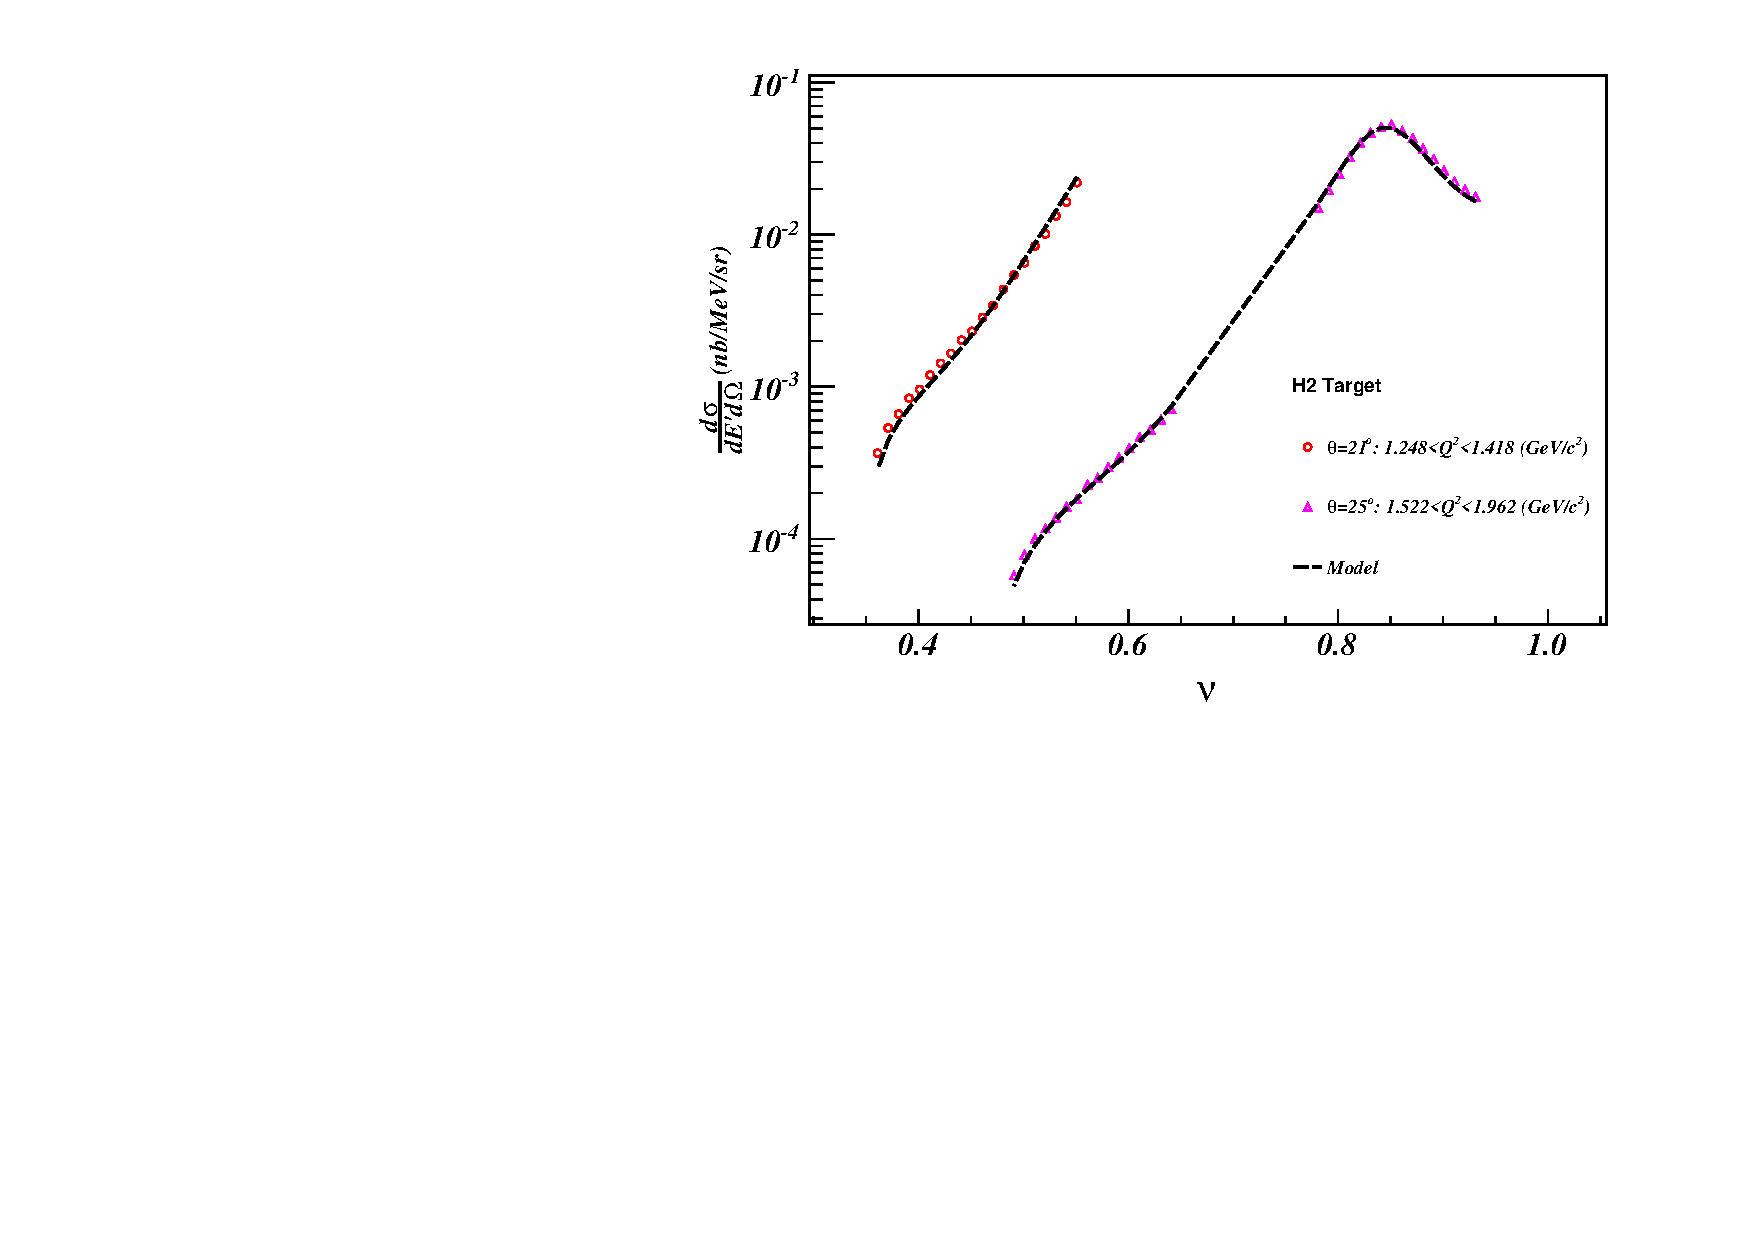
\includegraphics[type=pdf,ext=.pdf,read=.pdf,width=0.90\textwidth]{./figures/xs/H2_XS_All}
    }
    \\
    \subfloat[$\sigma^{^{2}H}_{born}$ .vs. $x_{bj}$]{
      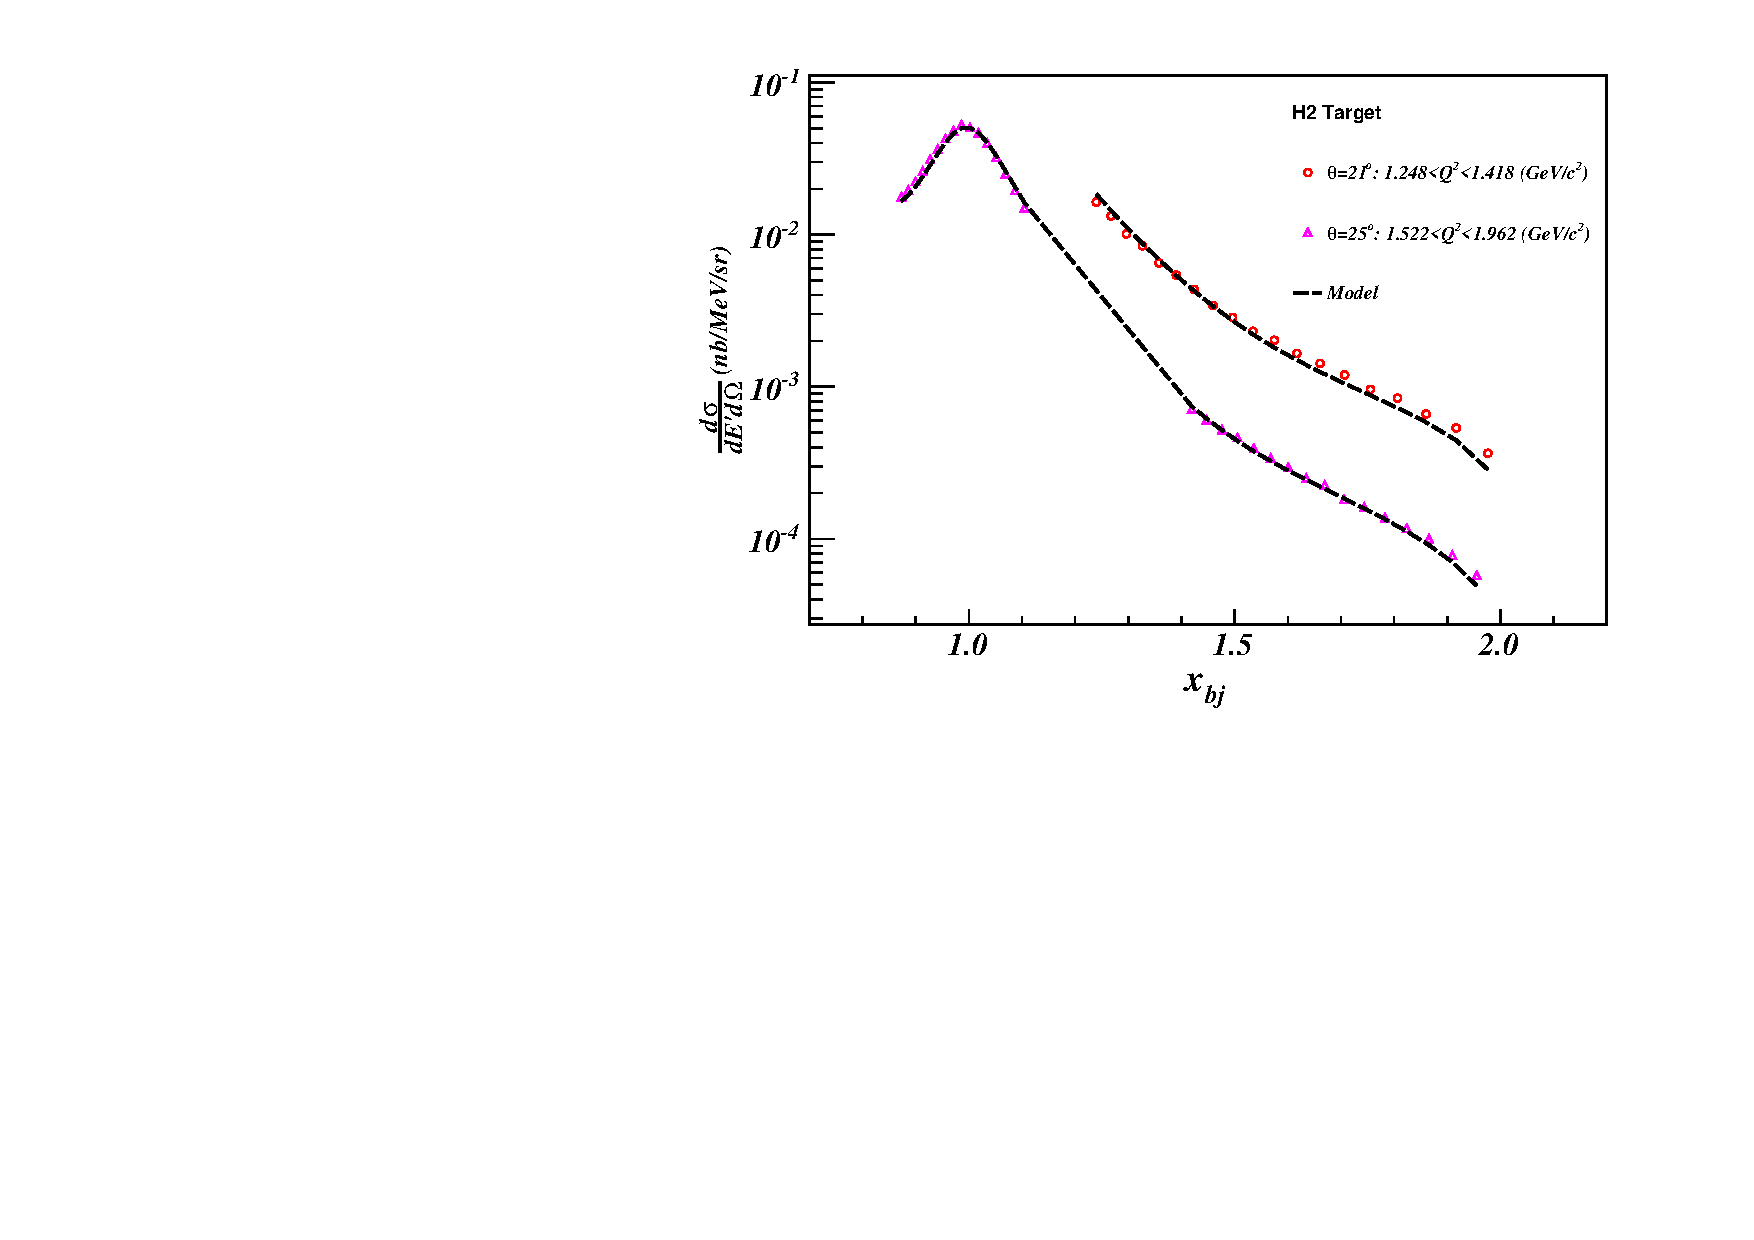
\includegraphics[type=pdf,ext=.pdf,read=.pdf,width=0.90\textwidth]{./figures/xs/H2_XS_All_xbj}
    }
    \caption[$\mathrm{^{2}H}$ preliminary born cross sections]{\footnotesize{$\mathrm{^{2}H}$ preliminary born cross sections, where dots are from experimental results and lines are calculated from XEMC model}}
    \label{xs_born_h2}
  \end{center}
\end{figure}
\begin{figure}[!ht]
  \begin{center}
    \subfloat[$\sigma^{^{3}He}_{born}$ .vs. $\nu$]{
      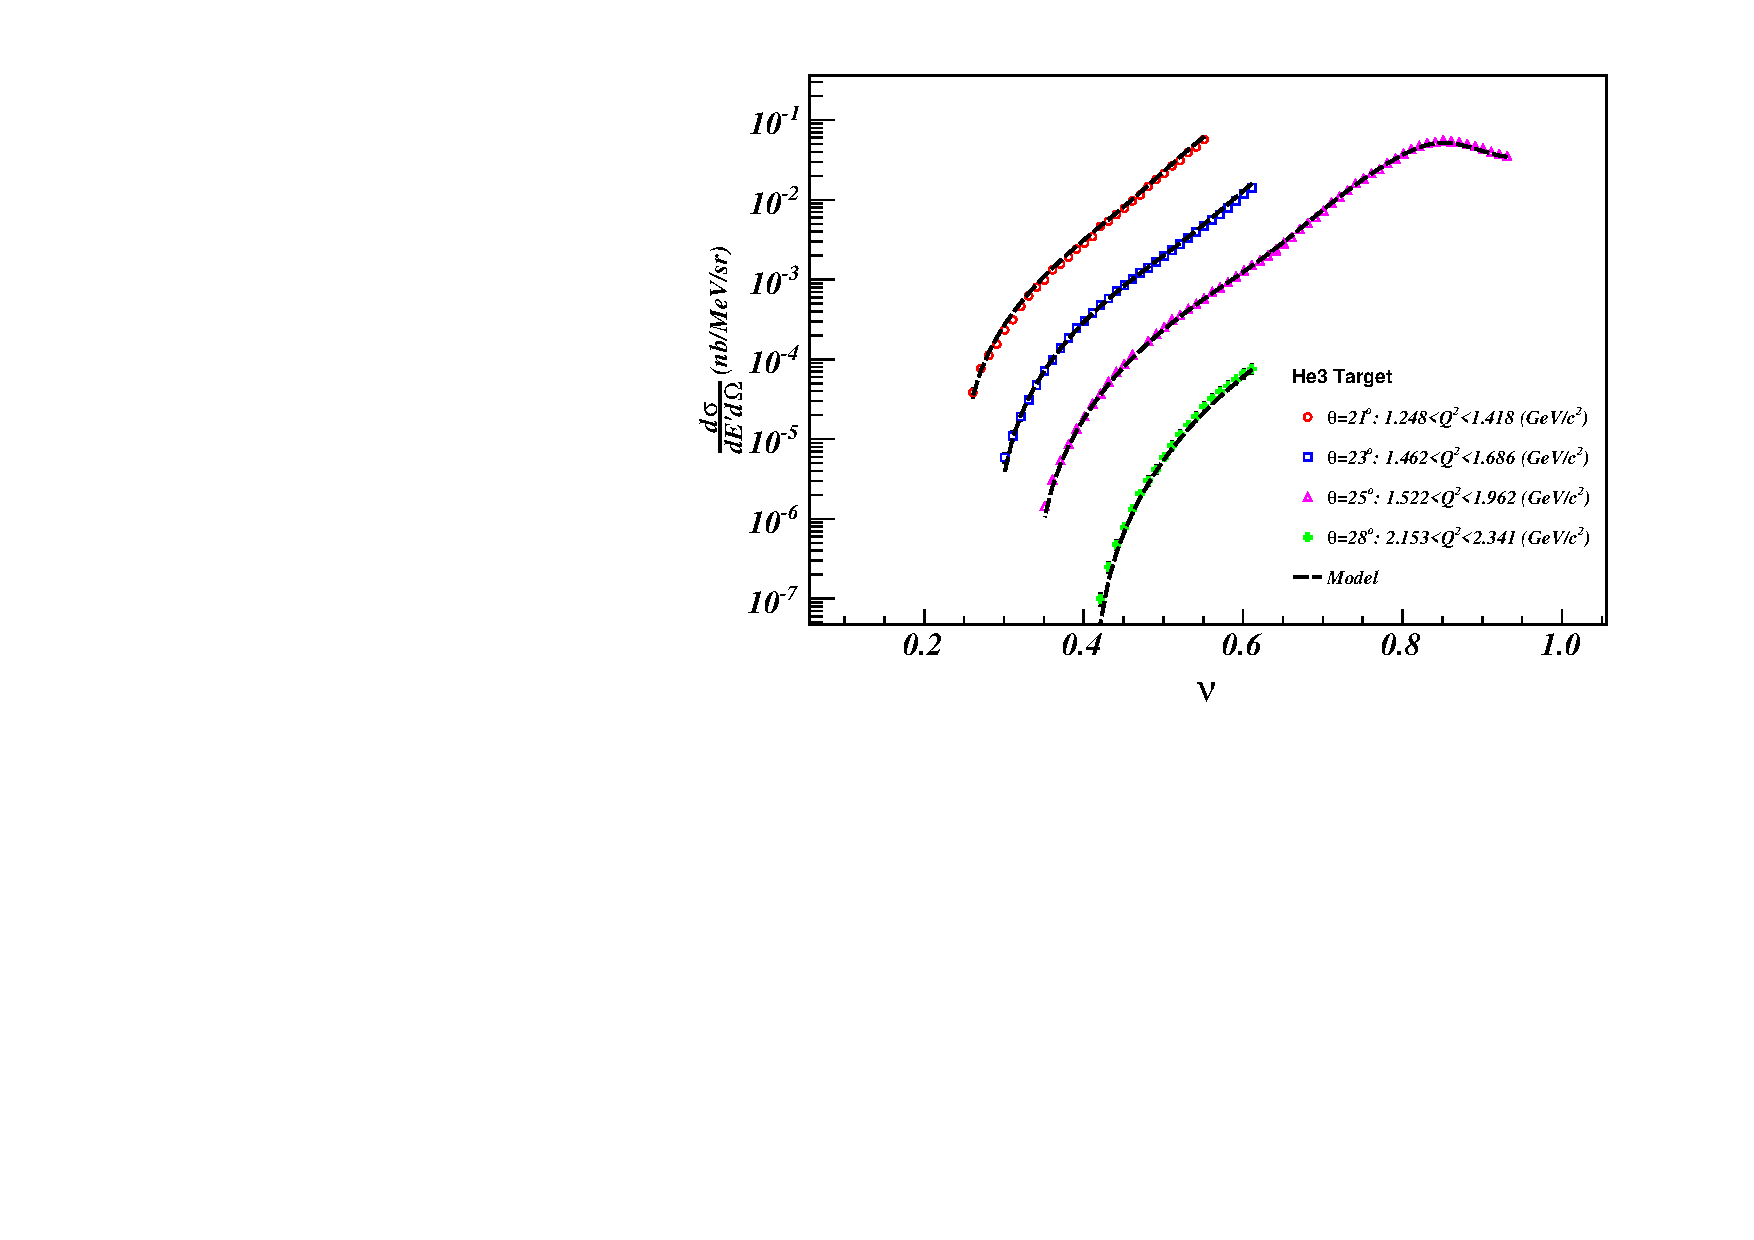
\includegraphics[type=pdf,ext=.pdf,read=.pdf,width=0.90\textwidth]{./figures/xs/He3_XS_All}
    }
    \\
    \subfloat[$\sigma^{^{3}He}_{born}$ .vs. $x_{bj}$]{
      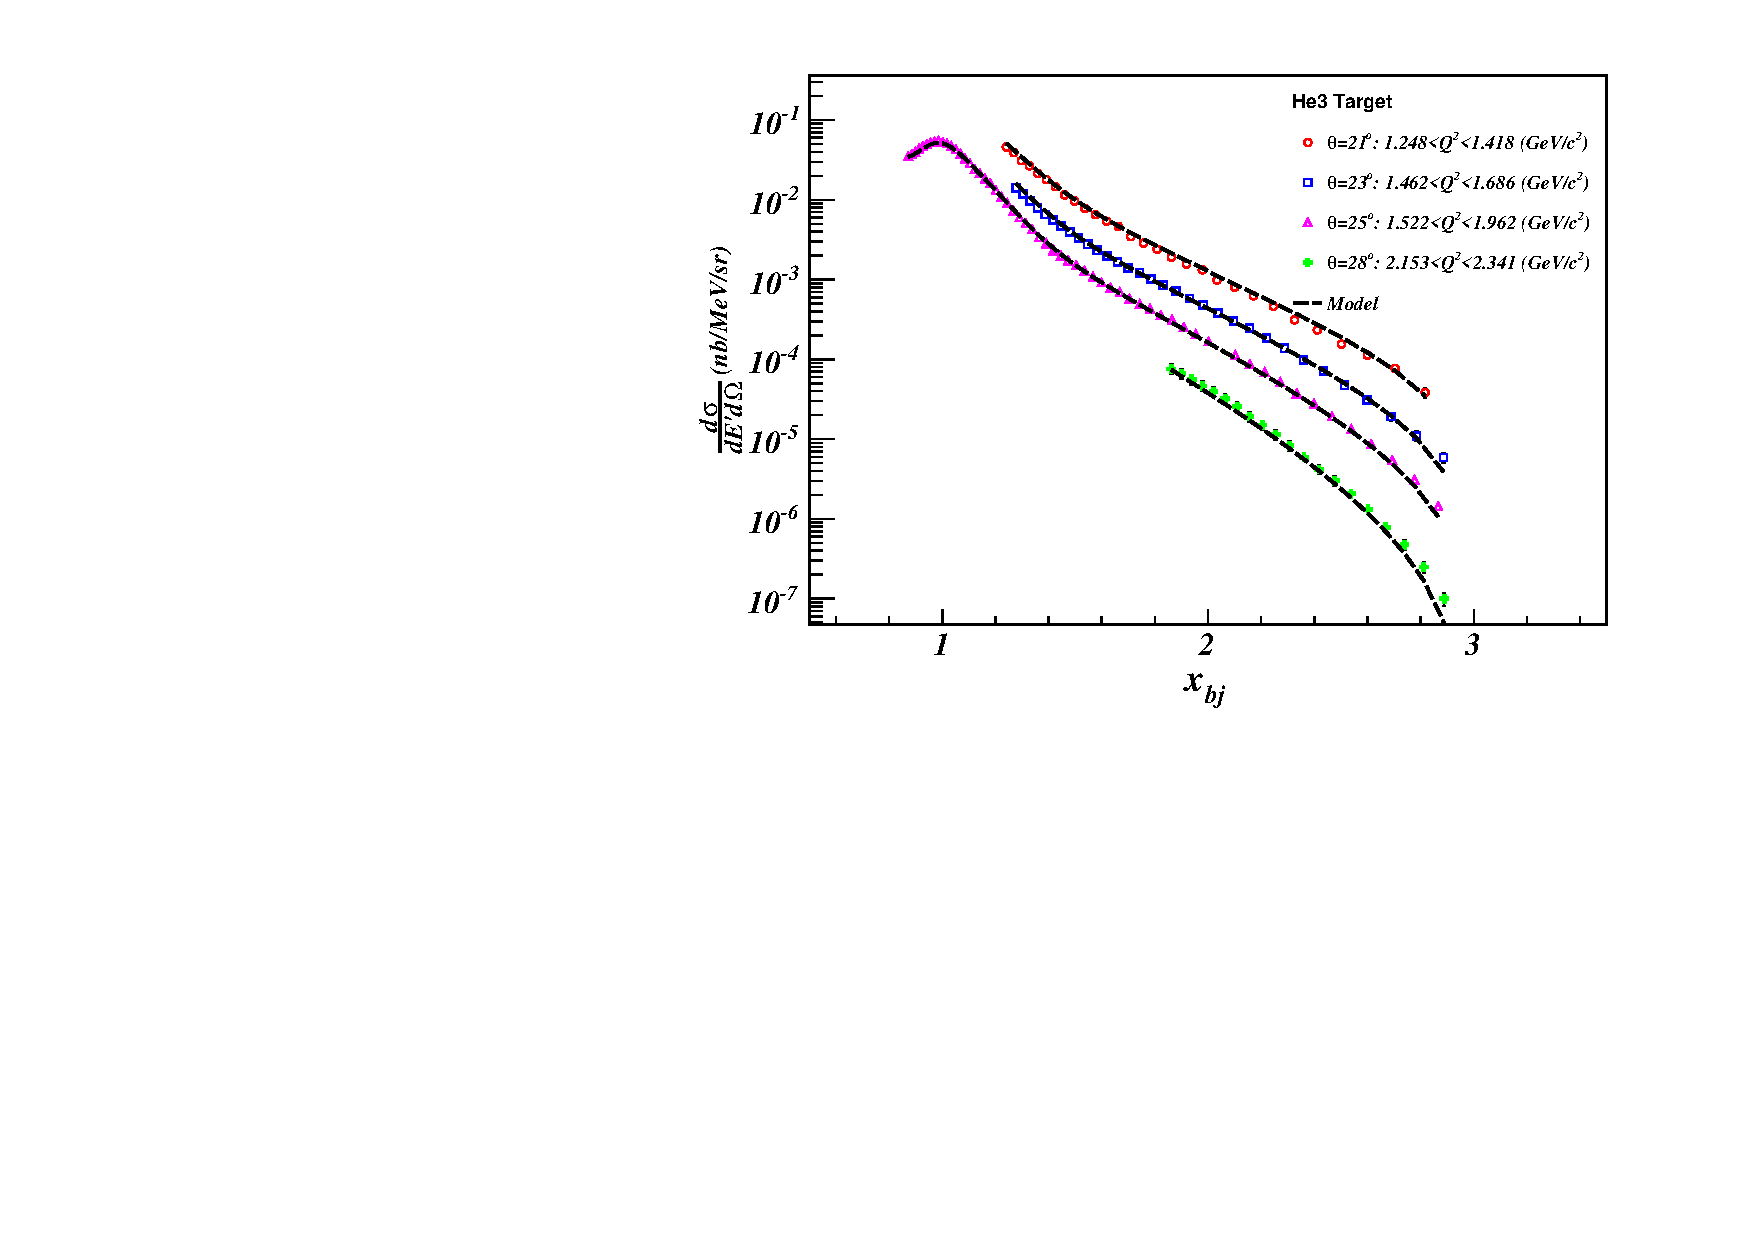
\includegraphics[type=pdf,ext=.pdf,read=.pdf,width=0.90\textwidth]{./figures/xs/He3_XS_All_xbj}
    }
    \caption[$\mathrm{^{3}He}$ preliminary born cross sections]{\footnotesize{$\mathrm{^{3}He}$ preliminary born cross sections, where dots are from experimental results and lines are calculated from XEMC model}}
    \label{xs_born_he3}
  \end{center}
\end{figure}
  \begin{figure}[!ht]
  \begin{center}
    \subfloat[$\sigma^{^{4}He}_{born}$ .vs. $\nu$]{
      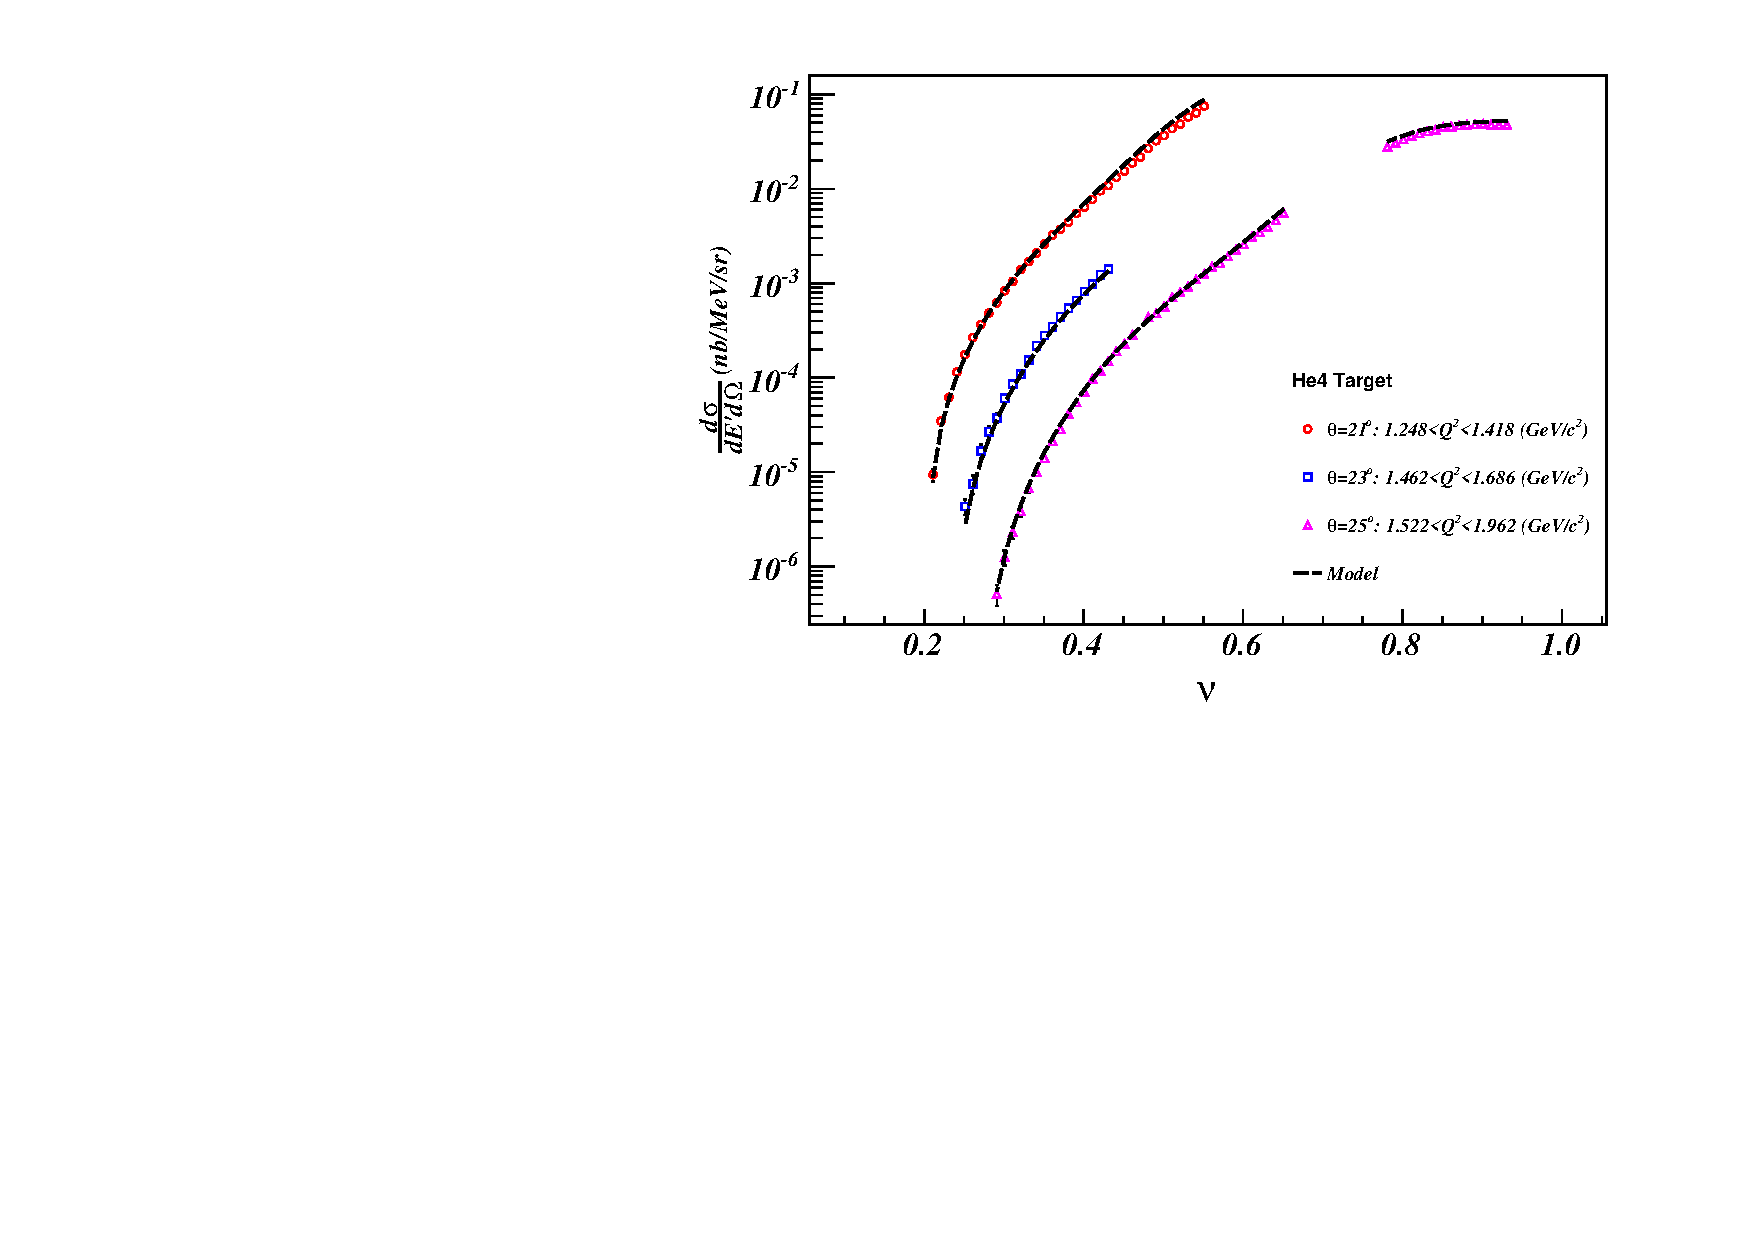
\includegraphics[type=pdf,ext=.pdf,read=.pdf,width=0.90\textwidth]{./figures/xs/He4_XS_All}
    }
    \\
    \subfloat[$\sigma^{^{4}He}_{born}$ .vs. $x_{bj}$]{
      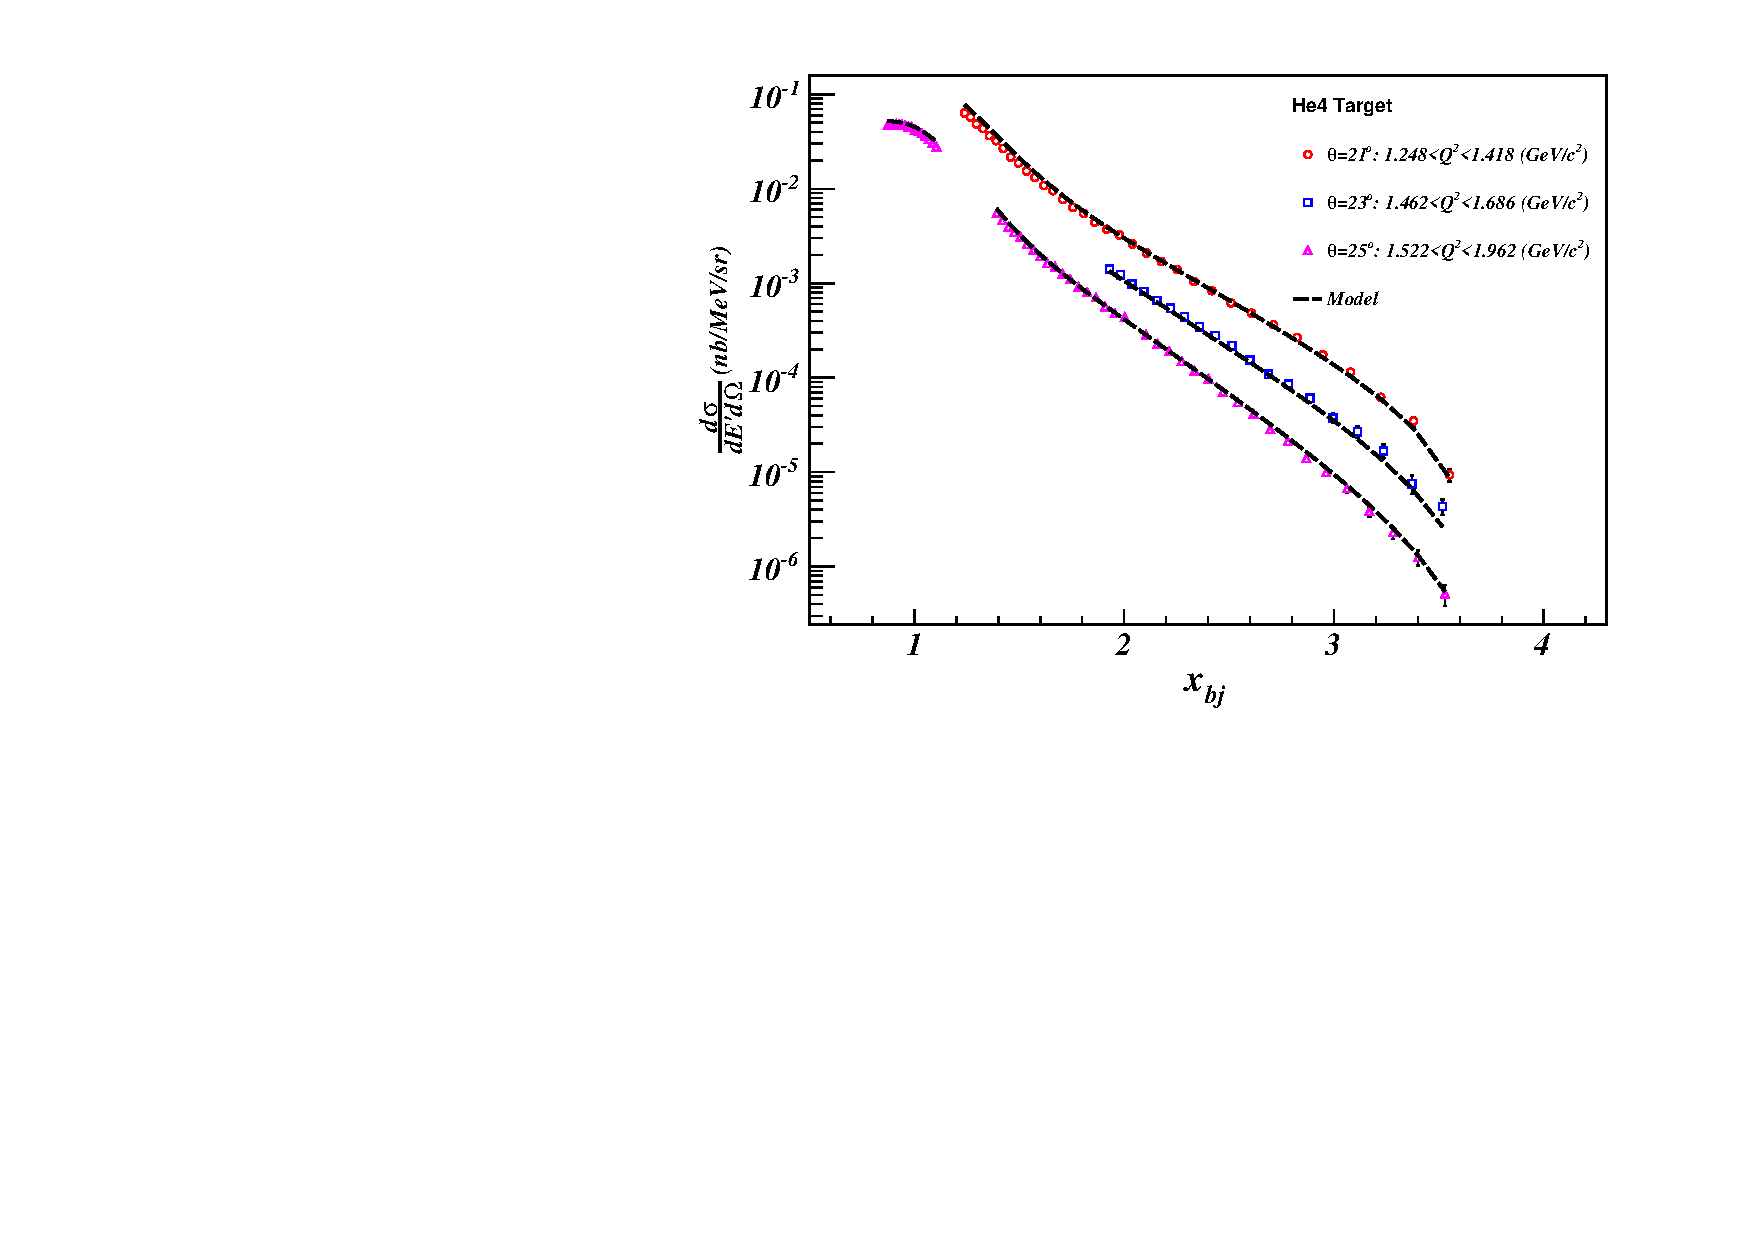
\includegraphics[type=pdf,ext=.pdf,read=.pdf,width=0.90\textwidth]{./figures/xs/He4_XS_All_xbj}
    }
    \caption[$\mathrm{^{4}He}$ preliminary born cross sections]{\footnotesize{$\mathrm{^{4}He}$ preliminary born cross sections, where dots are from experimental results and lines are calculated from XEMC model}}
    \label{xs_born_he4}
  \end{center}
\end{figure}

  \begin{figure}[!ht]
  \begin{center}
    \subfloat[$\sigma^{^{12}C}_{born}$ .vs. $\nu$]{
      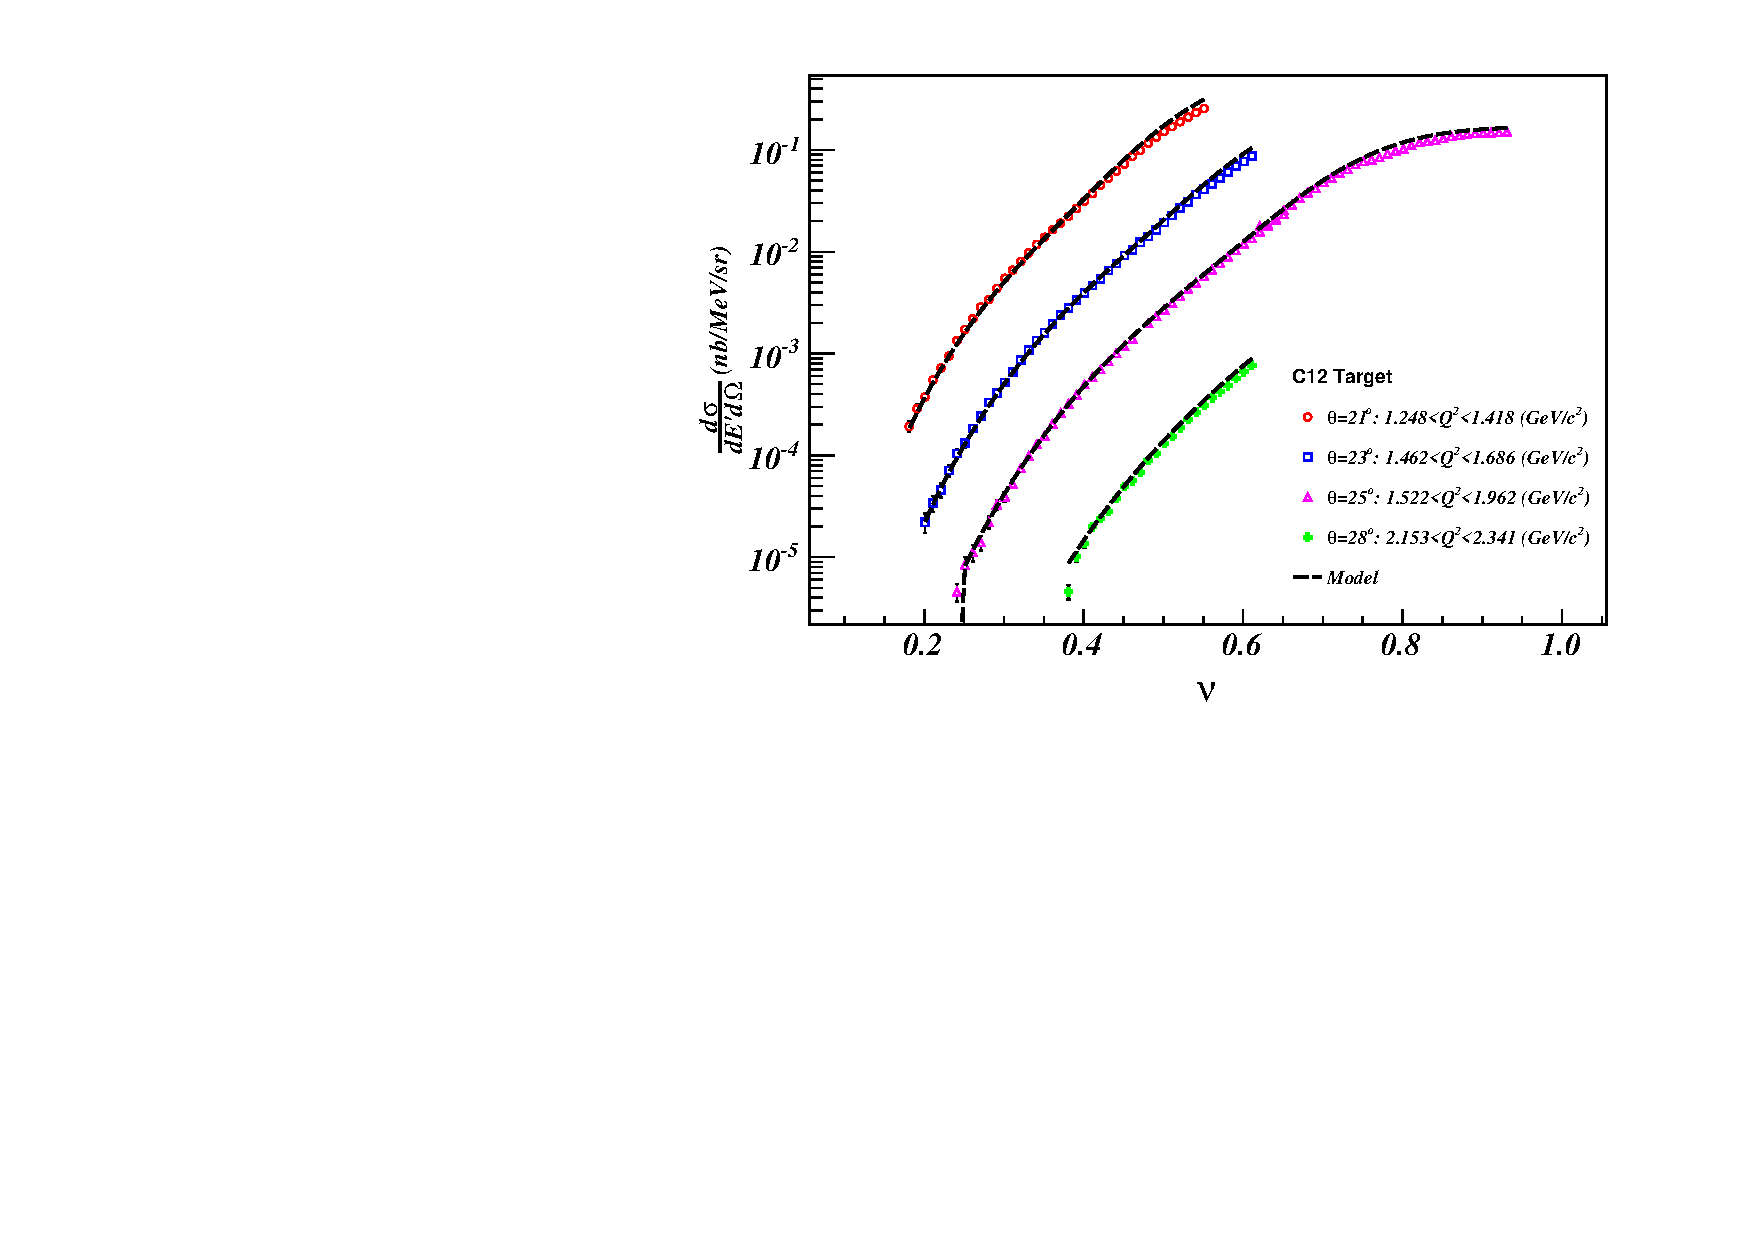
\includegraphics[type=pdf,ext=.pdf,read=.pdf,width=0.90\textwidth]{./figures/xs/C12_XS_All}
    }
    \\
    \subfloat[$\sigma^{^{12}C}_{born}$ .vs. $x_{bj}$]{
      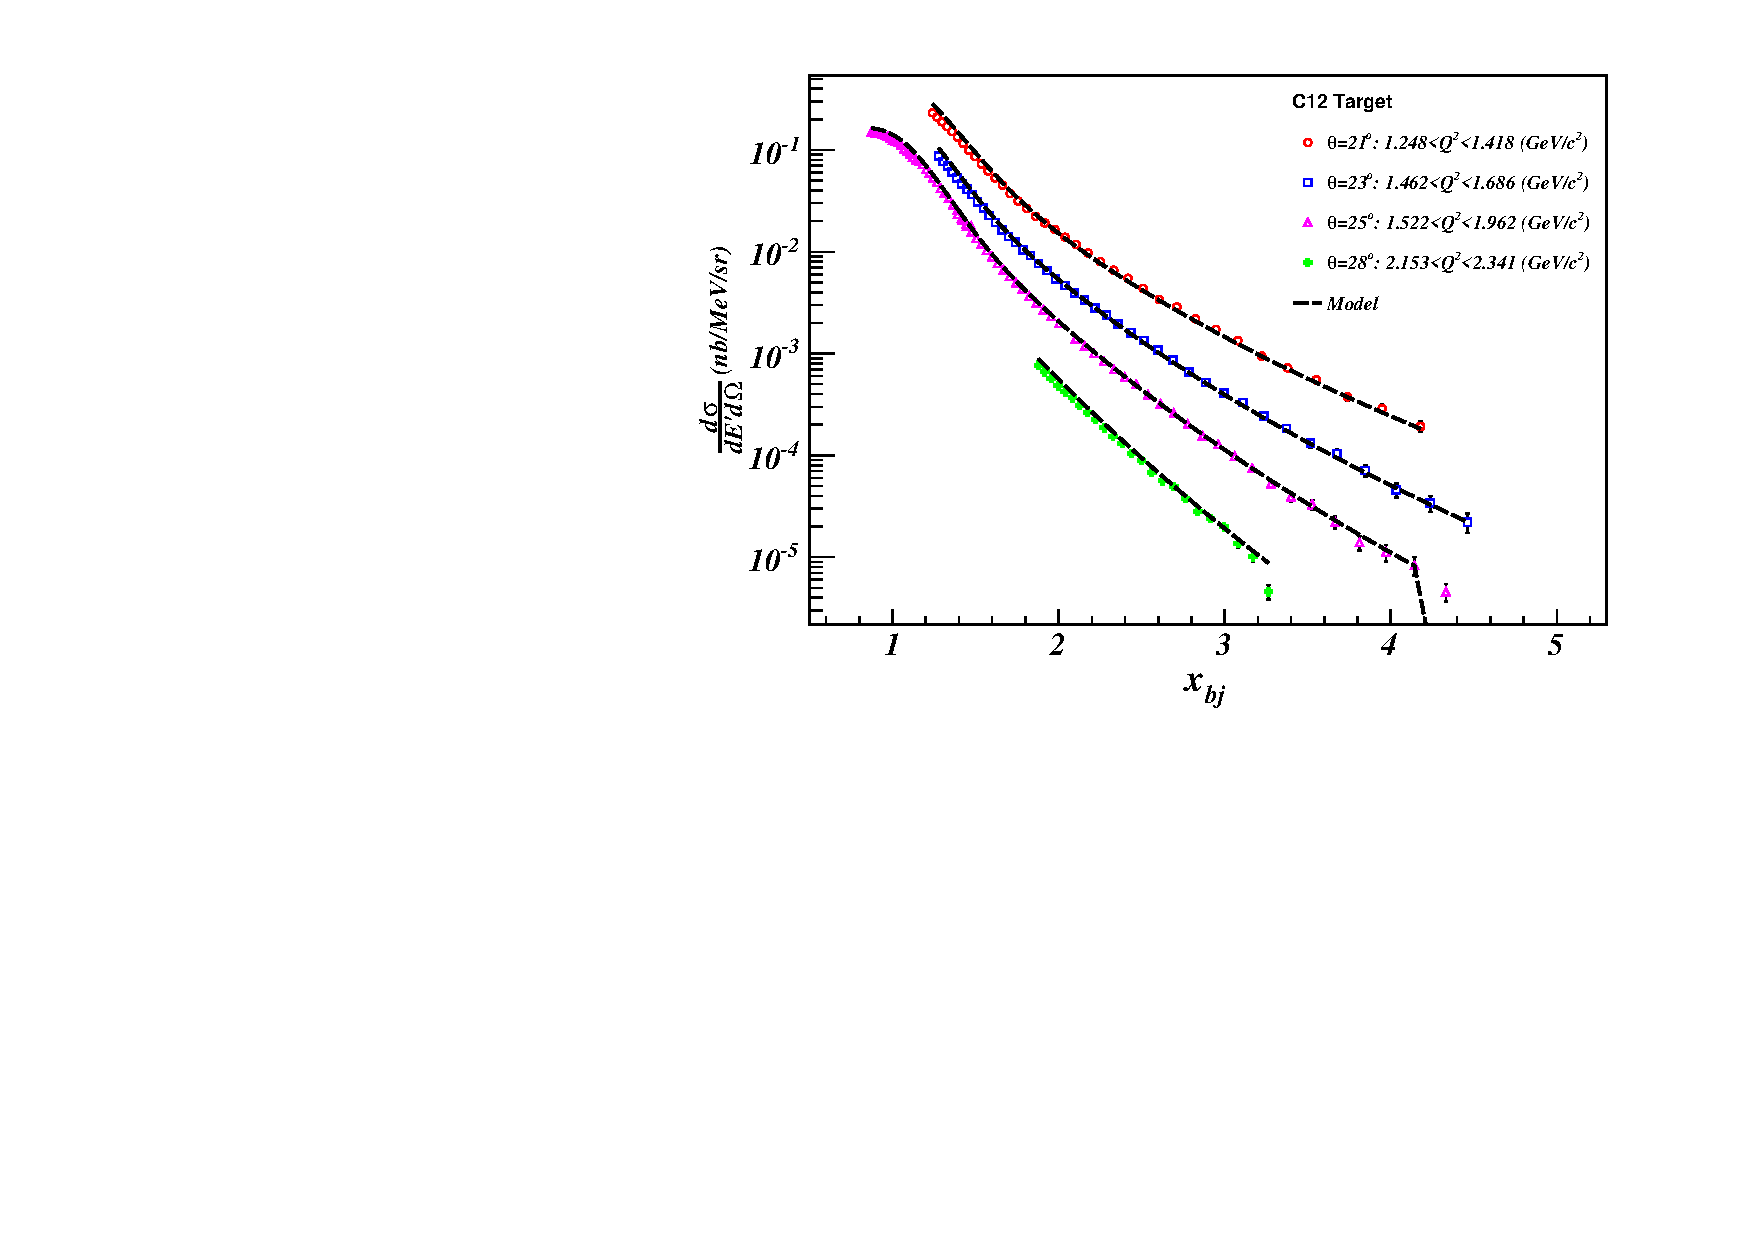
\includegraphics[type=pdf,ext=.pdf,read=.pdf,width=0.90\textwidth]{./figures/xs/C12_XS_All_xbj}
    }
    \caption[$\mathrm{^{12}C}$ preliminary born cross sections]{\footnotesize{$\mathrm{^{12}C}$ preliminary born cross sections, where dots are from experimental results and lines are calculated from XEMC model}}
    \label{xs_born_c12}
  \end{center}
\end{figure}

  \begin{figure}[!ht]
  \begin{center}
    \subfloat[$\sigma^{^{40}Ca}_{born}$ .vs. $\nu$]{
      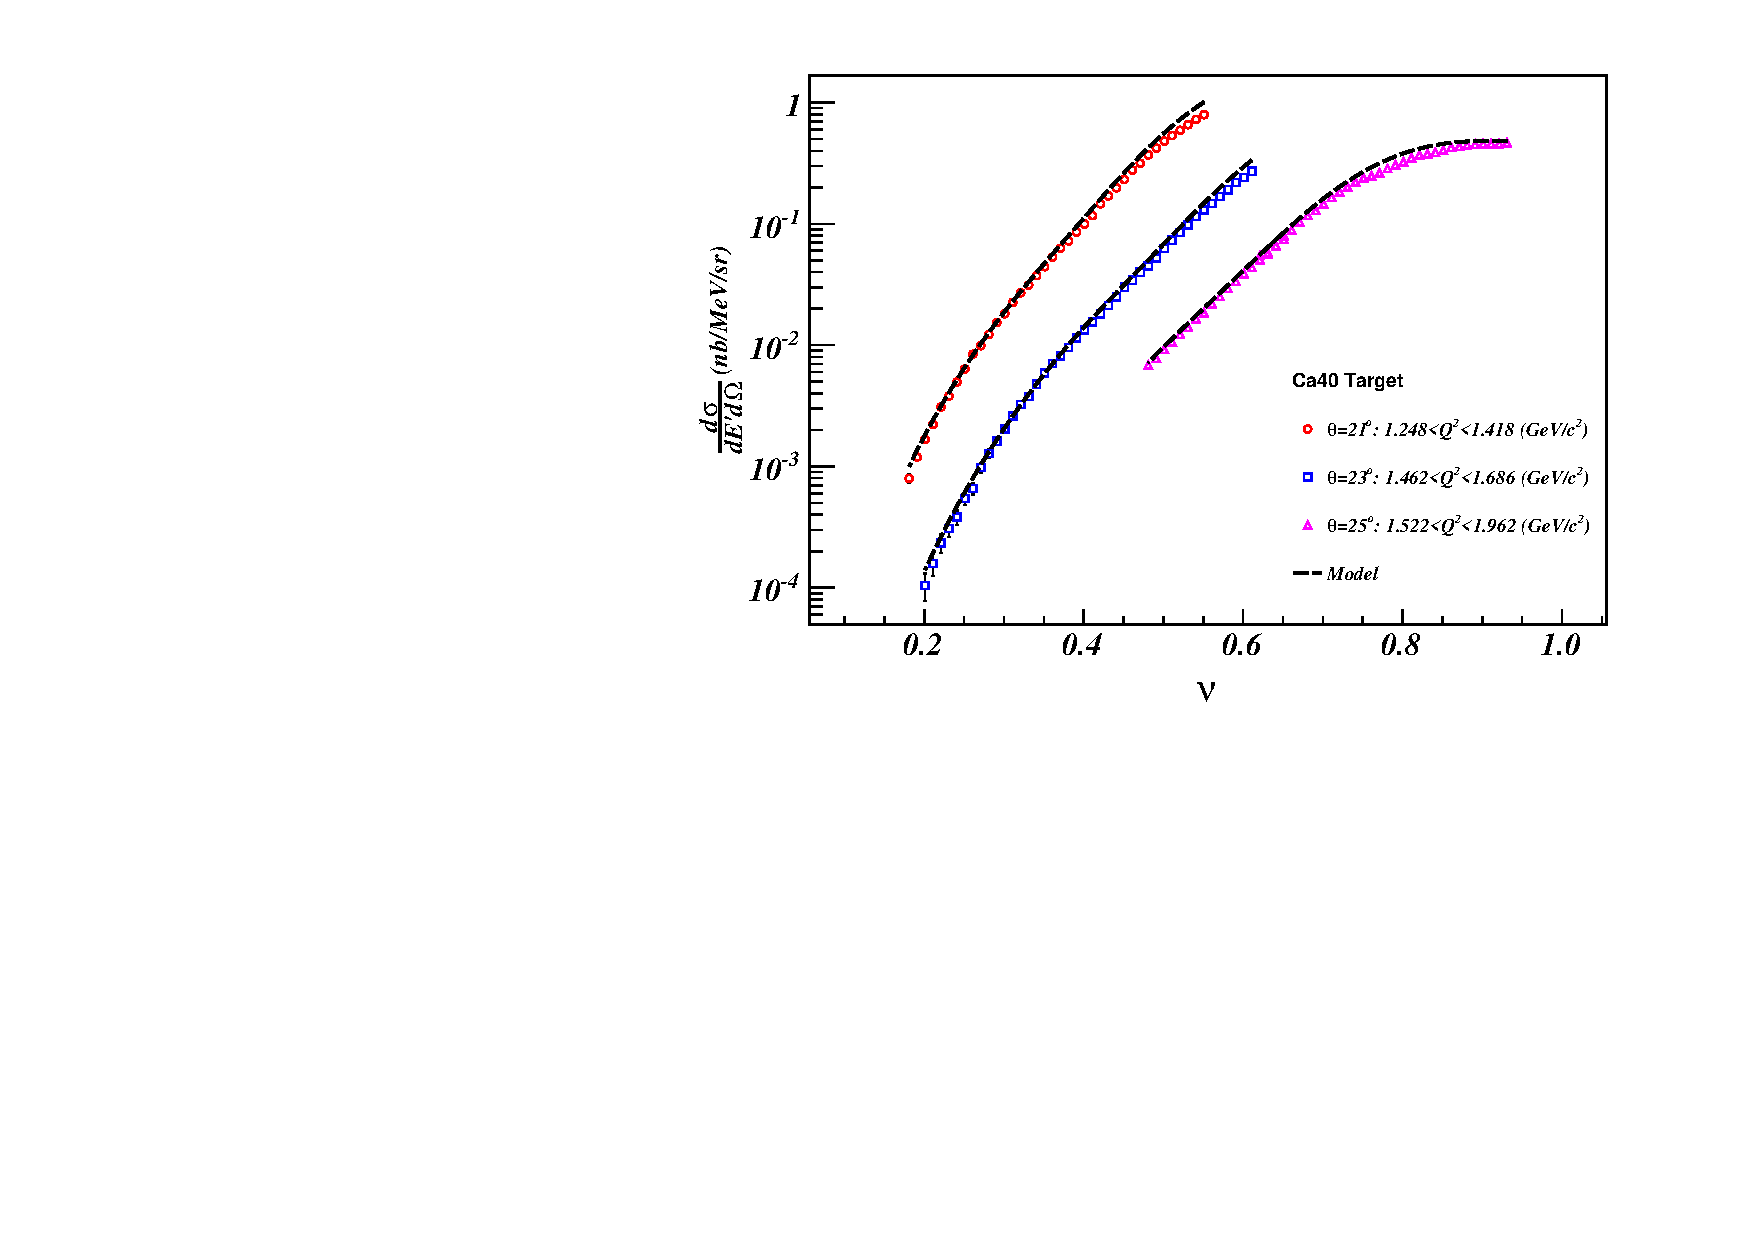
\includegraphics[type=pdf,ext=.pdf,read=.pdf,width=0.90\textwidth]{./figures/xs/Ca40_XS_All}
    }
    \\
    \subfloat[$\sigma^{^{40}Ca}_{born}$ .vs. $x_{bj}$]{
      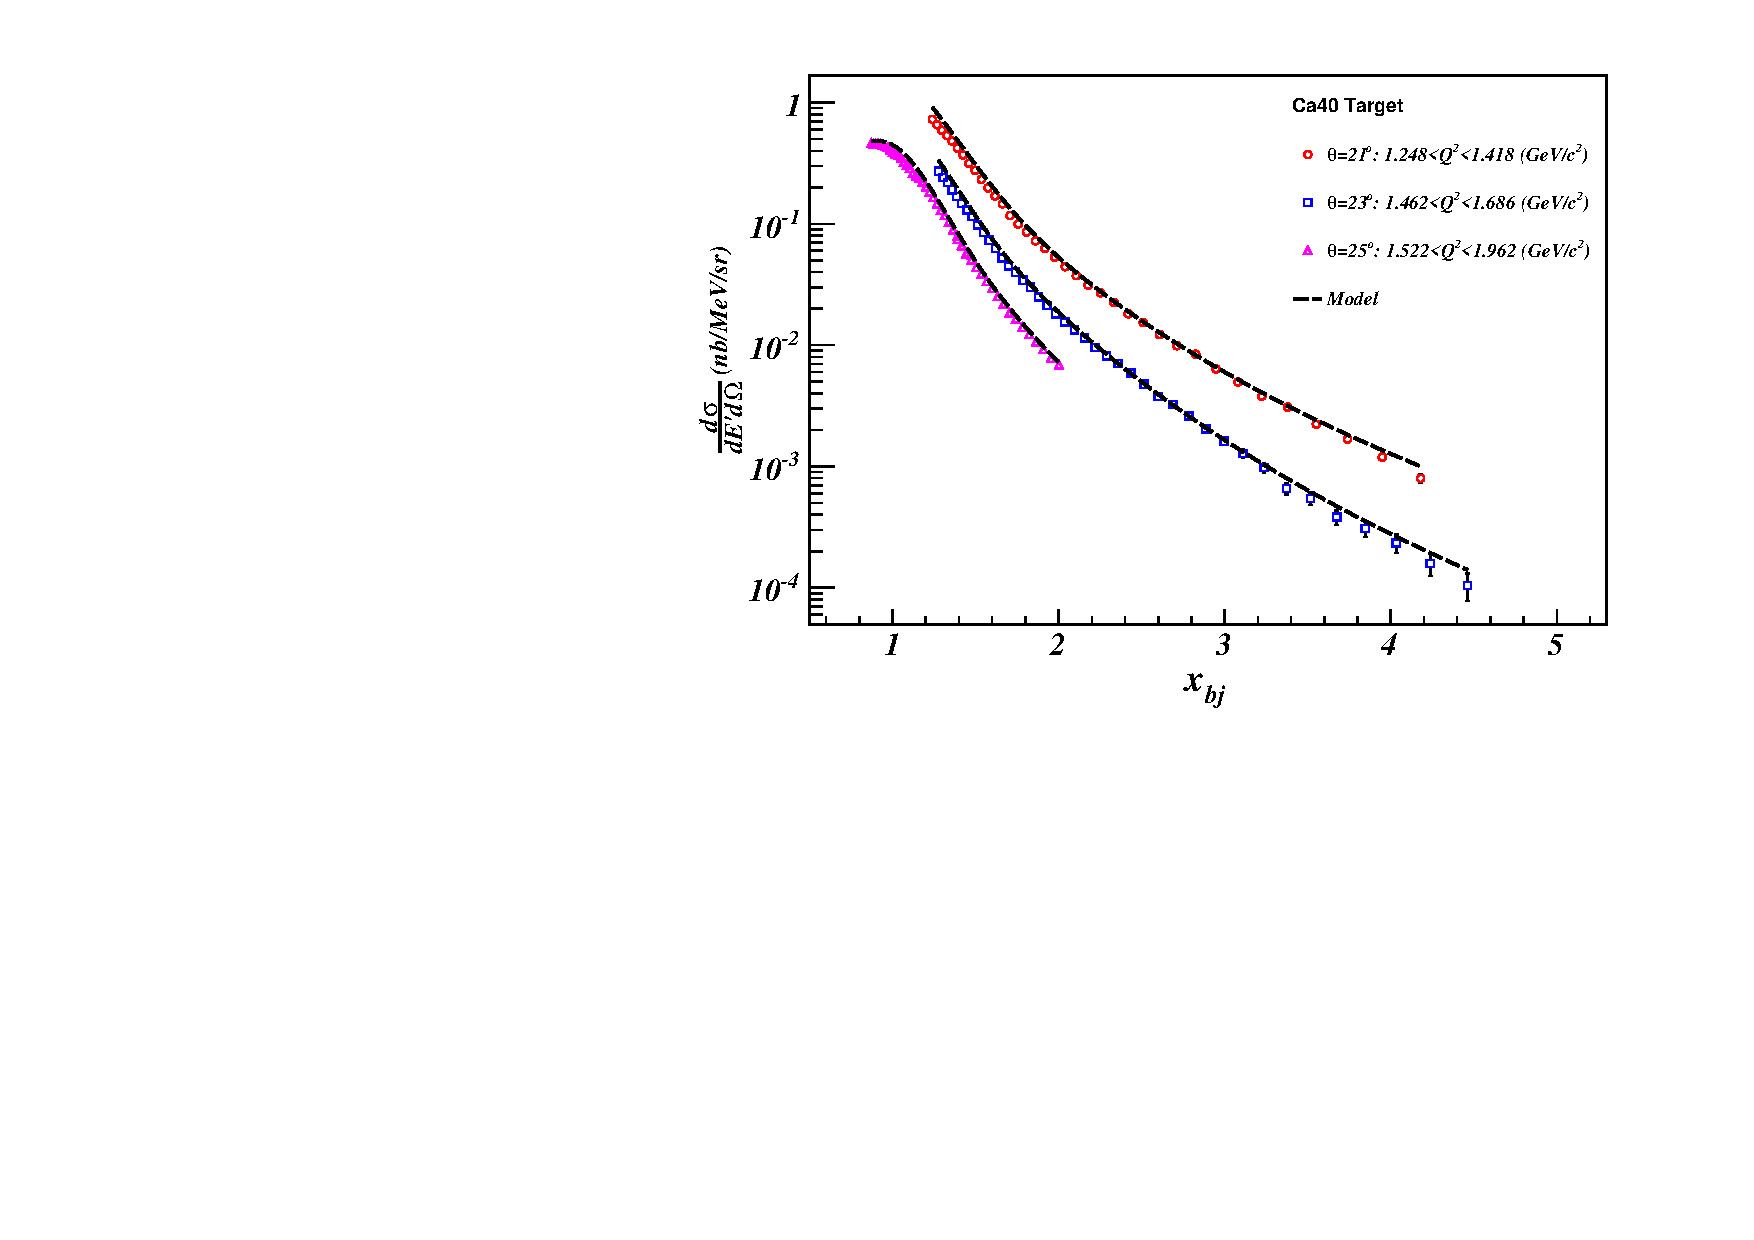
\includegraphics[type=pdf,ext=.pdf,read=.pdf,width=0.90\textwidth]{./figures/xs/Ca40_XS_All_xbj}
    }
    \caption[$\mathrm{^{40}Ca}$ preliminary born cross sections]{\footnotesize{$\mathrm{^{40}Ca}$ preliminary born cross sections, where dots are from experimental results and lines are calculated from XEMC model}}
    \label{xs_born_ca40}
  \end{center}
  \end{figure}
  
  \begin{figure}[!ht]
  \begin{center}
    \subfloat[$\sigma^{^{48}Ca}_{born}$ .vs. $\nu$]{
      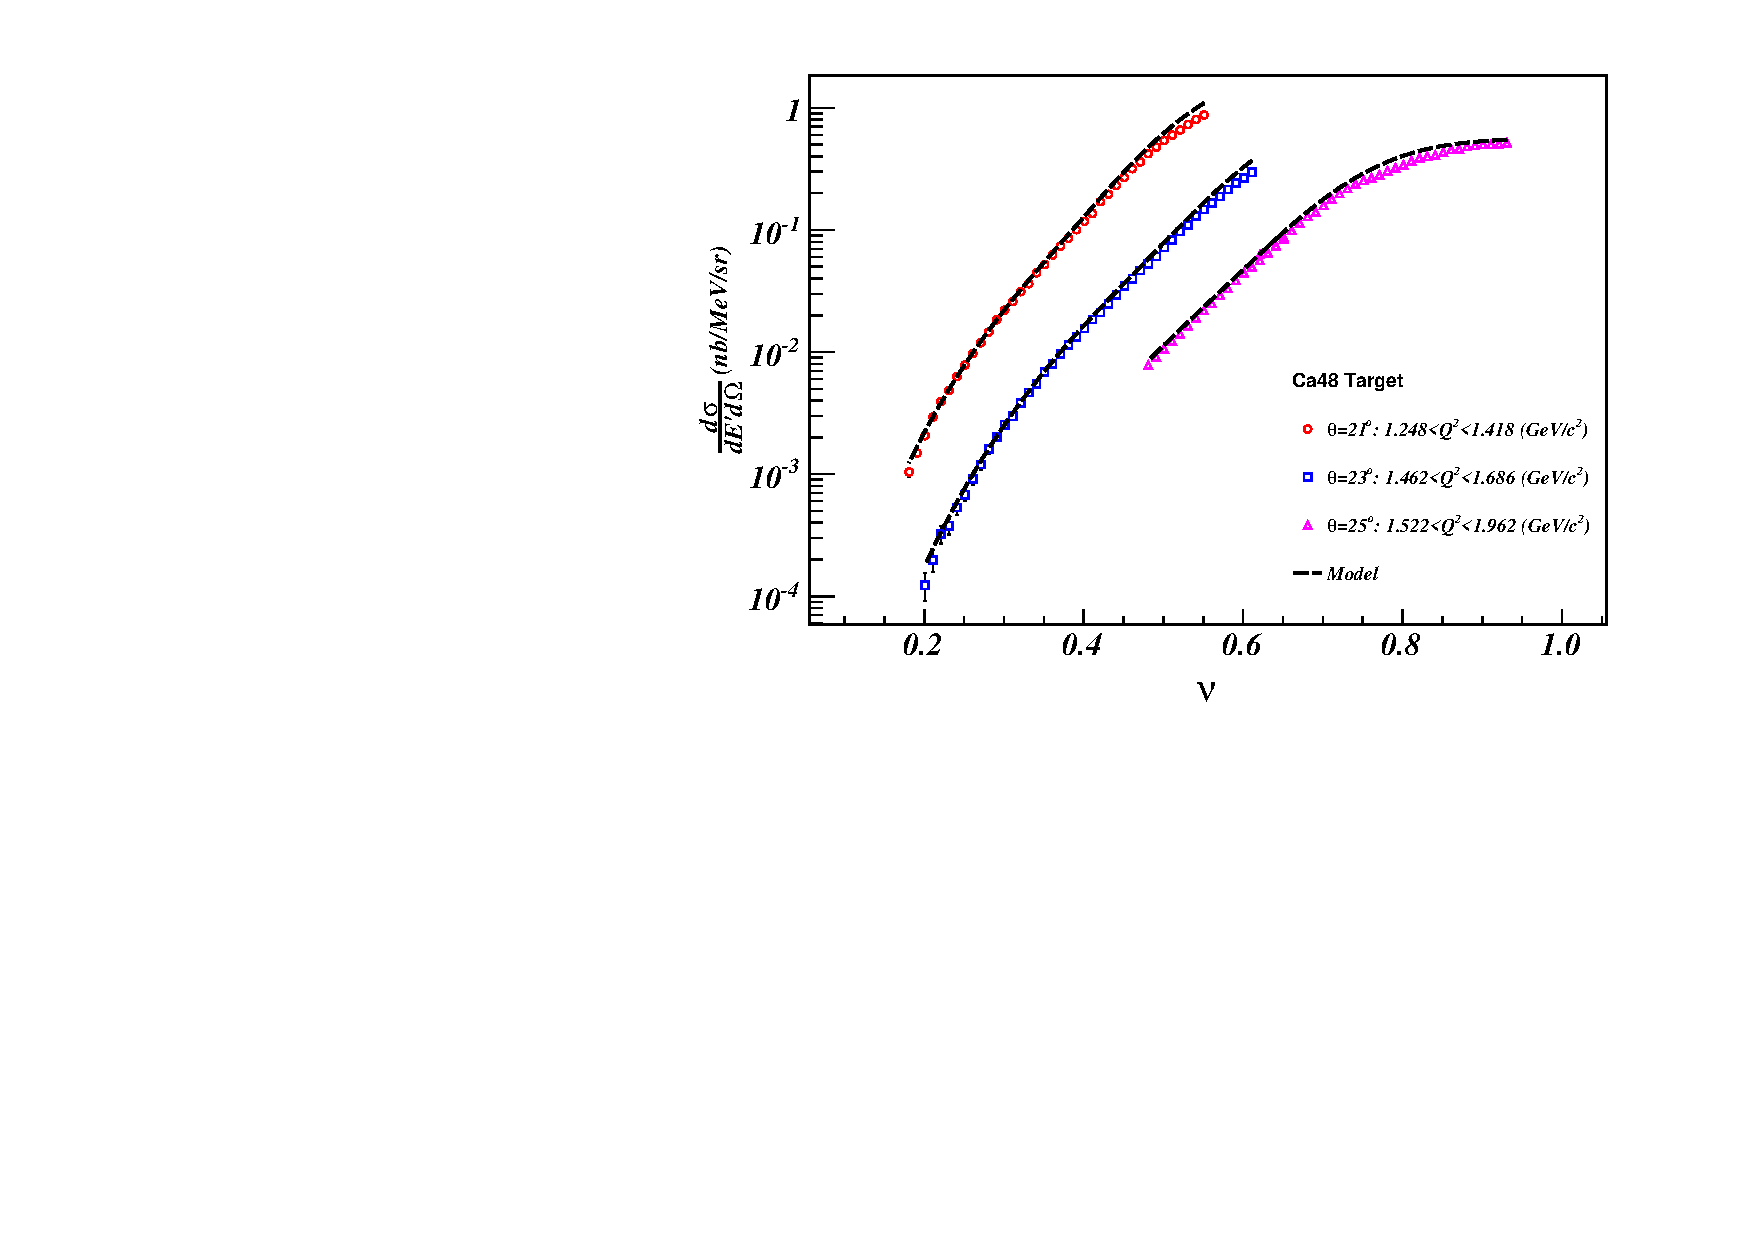
\includegraphics[type=pdf,ext=.pdf,read=.pdf,width=0.90\textwidth]{./figures/xs/Ca48_XS_All}
    }
    \\
    \subfloat[$\sigma^{^{48}Ca}_{born}$ .vs. $x_{bj}$]{
      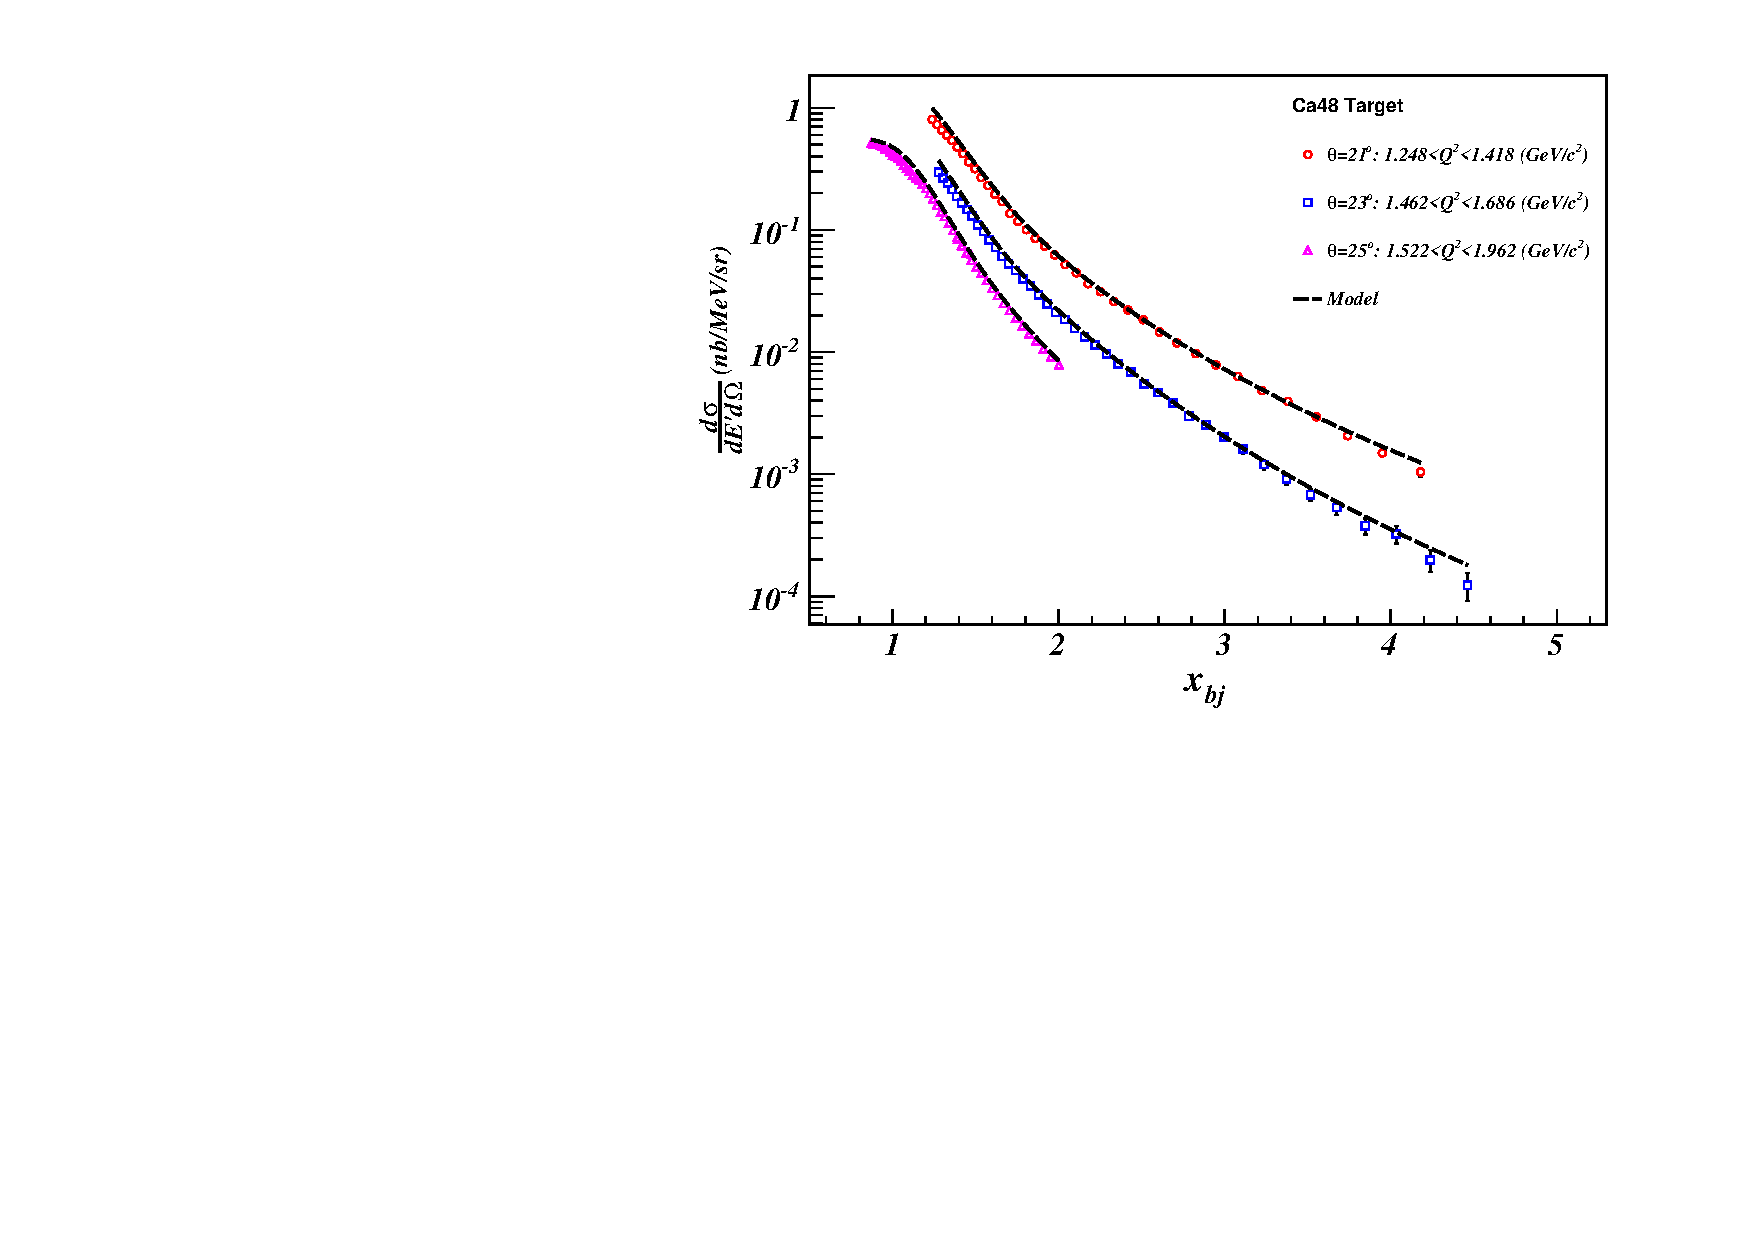
\includegraphics[type=pdf,ext=.pdf,read=.pdf,width=0.90\textwidth]{./figures/xs/Ca48_XS_All_xbj}
    }
    \caption[$\mathrm{^{48}Ca}$ preliminary born cross sections]{\footnotesize{$\mathrm{^{48}Ca}$ preliminary born cross sections, where dots are from experimental results and lines are calculated from XEMC model}}
    \label{xs_born_ca48}
  \end{center}
\end{figure}
%\section{Errors}
%The error bars shown here are calculated based on the discussion given in Chapter 5. 

%\begin{table}[!ht]
%  \centering
%  \begin{tabular}{|c|c|c|c|c|}
%    \hline
%    Source                   &  Scale   & Relative &  $\mathrm{\Delta\sigma/\sigma}$ & Comment\\
%    \hline\hline 
%    Trigger Efficiency       &  -       & 0.1\%    &                                 &        \\
%    Live-time                &  0.1\%   &  -       &                                 &        \\
%    VDC One-Track Efficiency &  0.4\%   & 0.3\%    &                                 &        \\
%    PID Efficiency           &  0.05\%  & 0.3\%    &                                 &        \\
%    \hline
%    Target Thickness         &0.5-2.4\% & -        &                                 &        \\
%    Beam Charge              &  0.4\%   & 0.3\%    &                                 &        \\
%    Beam Energy              & 0.05\%   & 0.02\%   &                                 &        \\
%    \hline
%    HRS-L Momentum           & 0.05\%   & 0.01\%   &                                 &        \\
%    HRS-L Angle              & 0.05\%   & 0.01\%   &                                 &        \\
%    HRS-R Momentum           & 0.05\%   & 0.01\%   &                                 &        \\
%    HRS-R Angle              & 0.05\%   & 0.01\%   &                                 &        \\
%    \hline    
%    Acceptance Correction    & 1\%      & 1\%      &                                 &        \\
%    Bin-Centering Correction & -        & 0.5\%    &                                 &        \\
%    Radiative Correction     & 1\%      & 1\%      &                                 &        \\
%    Coulomb Correction       & -        & 0-2\%    &                                 &        \\
%    \hline
%    Cryo-Target Boiling      &0.45\%    & 0.2\%    &                                 &        \\
%    Al End-Cups Subtraction  &$<$0.6\%  &0$\sim$1.8\% &                             &        \\
%    \hline
%   \end{tabular}
%  \caption[List of systematic errors]{List of systematic errors}
%  \label{stat_err_table}	
%\end{table}



